\chapter{Results}
\label{results}

%intro to the results
%below is a decent intro

%iterations of results - DIP, HIPPIE, Bayesian updating and reasoning behind it
% can then refer to this throughout this section.
As the project progressed the intended approach was found to be flawed and some changes were made.
%FIN: explain the flaws
The first of these was the change from a DIP-based training set to HIPPIE-based training set.
After the classification had been performed the use of a supervised classifier with this training set was found to be a poor method by itself for weighting interactions.
Using all of the data available it was possible to run a simple Bayesian alternative to continue with the weighting for the Community detection algorithm.

%Feature extraction results
\section{PPI feature vectors}

%The features extracted were X,Y,Z and the appendices explaining how this was done are A,B,C.
Many features were identified for extraction and these are described in Appendix \ref{datasources}.
Of these, only a small subset were succesfully processed into a usable form.
These can be found in appendix \ref{datasources}.

Of these, a smaller proportion were used in the final classifier, which neglected features directly derived from interaction databases.
The features used to train the final classifier are shown in table \ref{tab:features}.
A brief description of these features is given below.
%FIN: worth explaining wht the ENTS coverage is worse? 

%feature table, with information about each (size of features, categorical/ordinal/numerical, coverage)
\begin{table}
    \centering
    \small
    \begin{tabular}{l c c p{0.2\textwidth} p{0.2\textwidth}}
        Feature         &   Size &  Type                &  Coverage on training set &  Coverage on active zone network \\
        \hline
        Gene Ontology    &  90   &  Binary categorical  &  100.0\%                  & 100.0\%                          \\
        Yeast two-hybrid &  1    &  Numerical           &  100.0\%                  & 100.0\%                          \\
        ENTS derived     &  107  &  Numerical           &  38.39\%                  & 42.74\%                          \\
    \end{tabular}
    \caption{A table summarising the components of the feature vectors used in the final classifier.}
    \label{tab:features}
\end{table}

%these subsections may be too small
\subsection{Gene Ontology}
\label{go}

%Larger features
%Gene ontology was built as a feature in the same manner as that of qi_evaluation_2006 but, without knowing their approach, we had to develop our own method of creating usable features.
The Gene Ontology\autocite{ashburner_gene_2000} is a resource of annotations for genes to indicate various characteristics in a hierarchical manner, such as cellular localisation or function.
This resource has been used in past papers\autocite{qi_evaluation_2006} and in databases such as STRING\autocite{von_mering_string:_2005} to predict protein interactions.
Intuitively, it can be used to detect when, for example, two proteins are localised in the same area of the cell - as this would increase the probability that these two proteins interact.
%FIN: or rather is totally necessary for two proteins to interact in vivo even if they interact in vitro
%FIN: furthermore proteins which are known to share a function are intuitively more likely to interact than proteins of disparate function - for example proteins encoding consecutive steps in a biosynthetic pathway are often found to form complexes which stream-lines the synthesis of their product via biochemical channelling - directly passing the substrate to the active site of each protein without dealing with equilibria in the surrounding solution
Details on exactly how this feature was generated can be found in the notebook reference in Appendix \ref{app:go}.

\subsection{Features derived from ENTS}
\label{ents}
%ENTS features were retreived through analysis and modification of the code published on the ENTS website, but did not have full coverage on any dataset.

These features were obtained through analysis and modification of the bundled code and data downloaded from the website of \textcite{rodgers-melnick_predicting_2013}.
In turn, most of these features were generated through the Multiloc2 program of \textcite{blum_multiloc2:_2009}.
The remaining features are pairwise combinations of conserved protein domains, which are conserved "modules" of proteins described in \textcite{janin_domains_1985}.
%FIN: domains that can evolve independently as a discrete functional unit essentially 
%\subsection{Yeast Two-Hybrid results}
%\label{y2h}

%description of Y2H feature
%pending



\subsection{Data visualisation}
\label{dataviz}

%describe the problem of using in proportion and out of proportion methods
For all graphs, two cases were investigated: in proportion and out of proportion.
In proportion refers to the case where the proportion of interactions to non-interactions is correct; specifically, 1 interaction to 600 non-interactions.
%FIN: again justify Qi's basis for this ratio 
Out of proportion maintains the same number of interactions to non-interactions.
This is important as it is often easier to separated the data when the classes are equally split.
%FIN: why?

\subsubsection*{Reducing dimensionality}
%why do we want to reduce the dimensionality
If the data were two dimensional we would like to plot it as a scatter plot and see if there was a clear grouping of the points.
This would indicate that a classification algorithm would be able classify the data.
As the data has in excess of one hundred dimensions it is necessary to reduce the dimensionality before plotting.
%FIN: you could still use clustering algorithms in high dimension though 
%PCA is a relatively simply and fast way to reduce the high dimensionality of our feature vector into a form that can be easily plotted.
Two methods were tested to reduce the dimensionality of the data to two dimensions so that it could be easily plotted.
The first of these is PCA, which is relatively simple with a fast implementation, and the second is t-SNE, which is more complicated but has achieved better performance in recent works.
Both of these methods are described below in more detail.

%PCA description, referencing Barber
In PCA the method to express a high-dimensional point $\pmb{x}$ as a low dimensional point relies on finding an approximation for this point according to\autocite[330]{barber_bayesian_2013}:

%FIN: this kind of stuff seems more like methods than results to me 

\begin{align}
    \pmb{x}^{n} \approx \pmb{c} + \sum_{j=1}^{M} y_{j}^{n} \pmb{b}^{j} \equiv \tilde{\pmb{x}}^{n}
\end{align}

Where the low dimensional points are $\pmb{y}^{n}$, $\pmb{c}$ is a constant and $\pmb{b}_{j}$ are the principal components.
The algorithm to find these principal components is described in \textcite[333]{barber_bayesian_2013}.

The resulting plot produced using this technique is shown in figures \ref{fig:inpca} and \ref{fig:outpca} for the in proportion and out cases, respectively.
%FIN: typo/missing word

In the case of the data being out of proportion it appears that the groups can be separated.
However, this is not the case for the in proportion case.
%FIN: expand- make clear if this is a feature of your dataset or a case in general to do with prop and out-of-prop 

%plots
\begin{figure}
%    \setlength\figureheight{3in}
%    \setlength\figurewidth{4in}
%    \InputIfFileExists{\imagedir/in.pca.tikz}{}{\textbf{!! Missing graphics !!}}
    \centering
    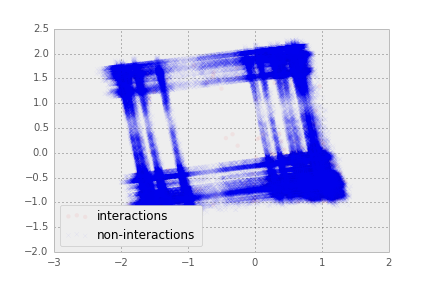
\includegraphics[width=0.6\textwidth]{in.pca.png}
    \caption{In proportion plot of the data reduced to two dimensions using PCA.}
    \label{fig:inpca}
\end{figure}

\begin{figure}
%    \setlength\figureheight{3in}
%    \setlength\figurewidth{4in}
%    \InputIfFileExists{\imagedir/out.pca.tikz}{}{\textbf{!! Missing graphics !!}}
    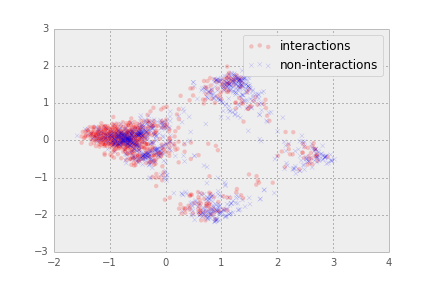
\includegraphics[width=0.6\textwidth]{out.pca.png}
    \centering
    \caption{Out of proportion plot of the data reduced to two dimensions using PCA.}
    \label{fig:outpca}
\end{figure}


%tSNE is more complicated, but was recommended due to reportedly good performance
A more complex method to reduce the dimensionality of the data is t-SNE\autocite{van_der_maaten_visualizing_2008}.
This technique won the Merck Visualization Challenge.   
It differs from PCA in the objective function in that it aims to maintain a similarity measure between points between the high and low-dimensional cases.

%should probably say what we did vis. TruncatedSVD
In addition to using this technique it was also recommended to use Truncated Singular Value Decomposition(SVD) to reduce the dimensionality of the vector to 50 beforehand.
%FIN: typo/missing word
%FIN: why was SVD recommended?

This was for implementation based reasons in Scikit-learn.
%FIN: typo/missing word

%results
Unfortunately, this was no more successful than PCA on this dataset, as shown in figures \ref{fig:intsne} and \ref{fig:outtsne}.
It should also be noted that the number of points plotted in these graphs is much lower than in the case of PCA as it is much more computationally intensive.
%FIN: because? 

%plots
\begin{figure}
%    \setlength\figureheight{3in}
%    \setlength\figurewidth{4in}
%    \InputIfFileExists{\imagedir/in.tsne.tikz}{}{\textbf{!! Missing graphics !!}}
    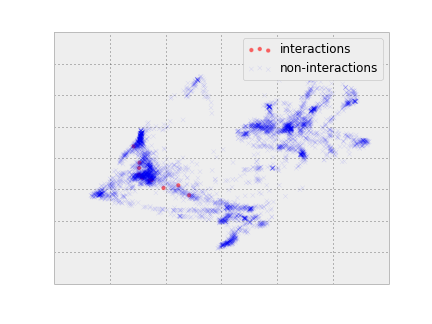
\includegraphics[width=0.6\textwidth]{in.tsne.png}
    \centering
    \caption{In proportion plot of the data reduced to two dimensions using t-SNE. Axes are not labeled as they are meaningless after the transformation.}
    \label{fig:intsne}
\end{figure}

\begin{figure}
%    \setlength\figureheight{3in}
%    \setlength\figurewidth{4in}
%    \InputIfFileExists{\imagedir/out.tsne.tikz}{}{\textbf{!! Missing graphics !!}}
    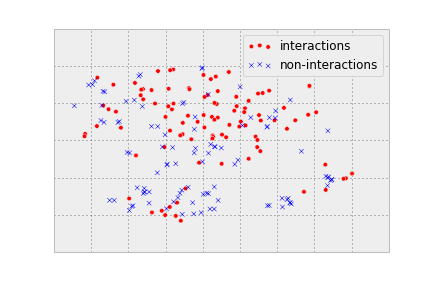
\includegraphics[width=0.6\textwidth]{out.tsne.png}
    \centering
    \caption{Out of proportion plot of the data reduced to two dimensions using t-SNE. Axes are not labeled as they are meaningless after the transformation.}
    \label{fig:outtsne}
\end{figure}

%Both methods show that this data is likely to be difficult to accurately categorize as the points are not separated in a 2d space
Both of the methods above suggest that this classification problem is difficult, as the points are not significantly separated in any of the plots.
%FIN: biology -- all continuous smears of things 

\subsection{High dimensional plots}

%Very few graphs are able to integrate large numbers of dimensions in a meaningful way; parallel line graphs and Andrew's curves are the two we have applied.
Neglecting reducing the dimensionality of the data there are some plots which are able to illustrate a very large number of dimensions.
Two which have been applied in this project are parallel lines plots and Andrew's curves\autocite{andrews_plots_1972}.
Parallel lines plots are relatively simple in that each feature is simply scaled and plotted along the x axis at its index in the vector, producing a number of overlapping lines.
Andrew's curves are more complex, and the method is described below along with the results obtained.
%FIN: this definitely all belongs in methods gav
%parallel line plot results
The parallel lines plots are shown in proportion in figure \ref{fig:inparline} and out of proportion in figure \ref{fig:outparline}.
In either case, it is not clear whether the data easily separates into two classes.
The in proportion case in particular shown in figure \ref{fig:inparlines} is very difficult to separate into interactions and non-interactions.

%this should be a tikz plot
\begin{figure}
%    \setlength\figureheight{3in}
%    \setlength\figurewidth{4in}
%    \InputIfFileExists{\imagedir/in.parallel.lines.tikz}{}{\textbf{!! Missing graphics !!}}
    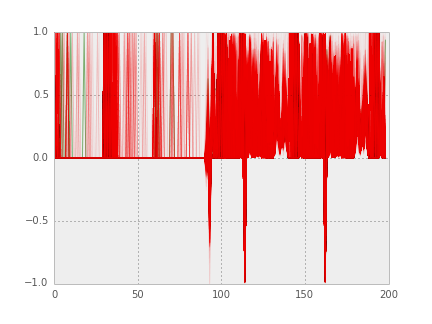
\includegraphics[width=0.6\textwidth]{in.parallel.lines.png}
    \centering
    \caption{In proportion parallel line plot of the data used to train the final classifier. Each feature vector is scaled into the graph interval and plotted, overlapping.}
    \label{fig:inparline}
\end{figure}

%this should be a tikz plot
\begin{figure}
%    \setlength\figureheight{3in}
%    \setlength\figurewidth{4in}
%    \InputIfFileExists{\imagedir/out.parallel.lines.tikz}{}{\textbf{!! Missing graphics !!}}
    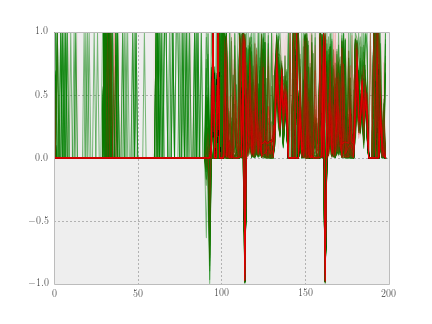
\includegraphics[width=0.6\textwidth]{out.parallel.lines.png}   
    \centering
    \caption{Out of proportion parallel line plot of the data used to train the final classifier. Each feature vector is scaled into the graph interval and plotted, overlapping.}
    \label{fig:outparline}
\end{figure}

%Explain how Andrew's curves work, what they mean.
%Andrew's curves are similar to parallel line plots in that they consist of overlapping lines.
%The lines in Andrew's curves are generated by mixing waves at different frequencies weighted based on the values of the features in the vector\autocite{andrews_plots_1972}.
%The result is a periodic wave that is modulated based on the values of the feature vectors.
%If the feature vectors of each class have reliably different values this should be reflected in the grouping of these curves.
%The two cases of in proportion and out are shown in figures \ref{fig:inandcurve} and \ref{fig:outandcurve}, respectively.
%
%\begin{figure}
%    \centering
%%    \setlength\figureheight{3in}
%%    \setlength\figurewidth{4in}
%%    \InputIfFileExists{\imagedir/in.andrews.curves.tikz}{}{\textbf{!! Missing graphics !!}}
%    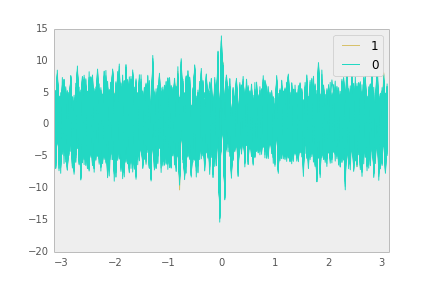
\includegraphics[width=0.6\textwidth]{in.andrews.curves.png}
%    \caption{In proportion Andrew's curves plot of the data used to train the final classifier.}
%    \label{fig:inandcurve}
%\end{figure}
%
%\begin{figure}
%    \centering
%%    \setlength\figureheight{3in}
%%    \setlength\figurewidth{4in}
%%    \InputIfFileExists{\imagedir/out.andrews.curves.tikz}{}{\textbf{!! Missing graphics !!}}
%    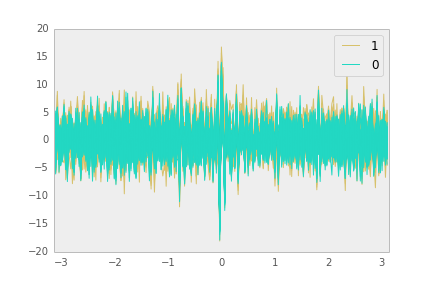
\includegraphics[width=0.6\textwidth]{out.andrews.curves.png}
%    \caption{Out of proportion Andrew's curves plot of the data used to train the final classifier.}
%    \label{fig:outandcurve}
%\end{figure}
%
%%what is shown in the plots?
%In neither graph is it easy to see a grouping of the curves being plotted.
%This means that it is likely to be very difficult to accurately classify the vectors.

\section{Classification in weighted PPI networks}

%why is this different to regular classification
In a classification task there are two common components: a training set that is labeled and a set of data which the classifier is to be applied to, without labels.
This task is similar in that we have created a training set with labels and the active zone network forms a set of feature vectors that have no labels.
However, this does not accurately encode our prior knowledge of the active zone network interactions, which were picked for their likelihood to be true interactions.
%FIN:how were they picked? 
For this reason, in this application classification alone is not sufficient to solve the problem of creating accurate weights, driving the development of the technique described in section \ref{bayes}.
%FIN: typo/missing word

This section describes both the results of training the classifier as planned on the labeled training set and the results of the Bayesian method to weight the interactions of the active zone network.

%Accuracy as a simple measure of the performance of a classifier is difficult to interpret in the case of a heavily unbalanced classifier such as this.
\subsection{Classifier accuracy and best parameters}
\label{gridresults}

%Using grid searches over the following parameter ranges we were able to search for the optimal parameters for each of the classifiers tested.
Grid searches of hyper-parameter values were used to find the optimal combination.
%FIN: optimal combination of what (hyper-paramters presumably)?
The results of this search are shown in table \ref{tab:gridresults}.

%table of the best parameters obtained for each classifier.
\begin{table}
    \centering
    \tiny
    \begin{tabular}{p{0.2\textwidth} c c c c c}
        Classifier                                  & Hyper-parameter values    & Test set accuracy     & Training set accuracy          \\
        \hline
        Logistic Regression                         & C : $0.0215$              & $0.9984 \pm 3\e{-5}$  & $0.99847 \pm 2\e{-5}$ \\
        \multirow{3}{*}{\parbox{0.2\textwidth}{Support Vector Machine}}     & kernel: RBF               & \multirow{3}{*}{$0.9985 \pm$ N/A}    & \multirow{3}{*}{$0.99933 \pm 1.2\e{-4}$} \\
                                                    & Gamma: $10.0$             &                           &                               &                               &       \\
                                                    & C: $10.0$                 &                           &                               &                               &       \\
        \multirow{2}{*}{\parbox{0.2\textwidth}{Random Forest}}              & N estimators: $44$        & \multirow{2}{*}{$0.99837 \pm 3\e{-5}$} & \multirow{2}{*}{$0.99921 \pm 3\e{-5}$} \\
                                                    & Max features: $25$        &                           &                               &                               &       \\
        \multirow{2}{*}{\parbox{0.2\textwidth}{Extremely Randomized Trees}} & N estimators: $94$        & \multirow{2}{*}{$0.99837 \pm 3\e{-5}$} & \multirow{2}{*}{$0.99921 \pm 3\e{-5}$} \\
                                                    & Max features: $25$        &                           &                               &                               &       \\
    \end{tabular}
    \caption{Summary of the hyper-parameter combinations found by grid search and associated statistical accuracy measures.}
    \label{tab:gridresults}
\end{table}

Although the results of the Support Vector Machine appear to be good, it was trained on a relatively small dataset and its performance in later tests deemed it unsuitable to our classification task.
%FIN: in what way? you don't mention why you chose certain kernels

The random forest can be seen to be performing worse than the logistic regression model in this test, with a slightly lower accuracy, but within the standard error boundaries.
%FIN: any idea why? 


\subsection{ROC curves}

%A ROC curve plots the tradeoff between true positive and false positive rates, in the case of an unbalanced classifier large sample sizes are required to obtain a smooth, stable curve.
As described in section \ref{classifierverification} ROC curves were applied to all classifiers to characterise the performance of each.
The ROC curve produced by the logistic regression model is shown in figure \ref{fig:logroc}.
The positive AUC value is desirable and the curve of the ROC curve suggests this model can achieve a relatively good true positive rate at low false positive rate, which is likely what it would be used at - to avoid false positive protein interactions being classified.
%FIN: sentence too complex - split


%ROC curves for the different classifiers
%with AUC values in the captions
\begin{figure}
    \centering
    \setlength\figureheight{2in}
    \setlength\figurewidth{3in}
    \InputIfFileExists{\imagedir/logreg.roc.tikz}{}{\textbf{!! Missing graphics !!}}
    \caption{The ROC curve produced by a logistic regression model on the test data set using the best parameters shown in table \ref{tab:gridresults} with an AUC of $0.781$.}
    \label{fig:logroc}
\end{figure}

\begin{figure}
    \centering
    \setlength\figureheight{2in}
    \setlength\figurewidth{3in}
    \InputIfFileExists{\imagedir/rf.roc.tikz}{}{\textbf{!! Missing graphics !!}}
    \caption{The ROC curve produced by a random forest model on the test data set using the best parameters shown in table \ref{tab:gridresults} with an AUC of $0.806$.}
    \label{fig:rfroc}
\end{figure}

%commented out as graph is not worth including
%\begin{figure}
%    \centering
%    \setlength\figureheight{3in}
%    \setlength\figurewidth{4in}
%    \InputIfFileExists{\imagedir/svc.roc.tikz}{}{\textbf{!! Missing graphics !!}}
%    \caption{The ROC curve produced by a support vector machine model on the test data set using the best parameters shown in table \ref{tab:gridresults}.}
%    \label{fig:svcroc}
%\end{figure}

However, the ROC curve shown in figure \ref{fig:rfroc} is very similar to that created by the logistic regression model except it has slightly better performance at low false positive rates.
Neither show very good performance and it clear that only at very high false positive rates will the classifiers reliably find the true interactions.
%FIN: typo/missing word


Unfortunately, it was not possible to train the support vector machine on a large enough training set to plot a realistic ROC curve due to time constraints, so it is not shown here.
The notebook referenced in appendix \ref{app:classtrain} provides the results obtained.
This is also true of the precision-recall graph in the following section.

%differences between the classifiers and reasons for this.

\subsection{Precision-recall curves}

%what a precision recall plot is? already in methods
As described in section \ref{classifierverification} the classifiers were also characterised through plotting a precision-recall curve.
This is shown for the random forest and logistic regression models in figures \ref{fig:rfpr} and \ref{fig:logpr}, respectively.
Although the random forest model achieves a better AUC value, the curve demonstrates is unable to recall as many samples with perfect precision as the logistic regression model.
%FIN: typo/missing word

As with the ROC curve, neither classifier shows particularly good performance.
%FIN: be more positive - These results supported those acquired by the ROC analysis 

%precision recall curves for the different classifiers
\begin{figure}
    \centering
    \setlength\figureheight{2in}
    \setlength\figurewidth{3in}
    \InputIfFileExists{\imagedir/logreg.pr.tikz}{}{\textbf{!! Missing graphics !!}}
    \caption{The precision-recall curve produced by a logistic regression model on the test data set using the best parameters shown in table \ref{tab:gridresults} with an AUC of $0.11$.}
    \label{fig:logpr}
\end{figure}

\begin{figure}
    \centering
    \setlength\figureheight{2in}
    \setlength\figurewidth{3in}
    \InputIfFileExists{\imagedir/rf.pr.tikz}{}{\textbf{!! Missing graphics !!}}
    \caption{The precision-recall curve produced by a random forest model on the test data set using the best parameters shown in table \ref{tab:gridresults} with an AUC of $0.12$. This graph shows some artefacts due to the extremely small number of positive interactions even in relatively large sample sizes.}
    \label{fig:rfpr}
\end{figure}

\subsection{Feature importances}
\label{importances}

%Comparing logistic regression to random forests
Both logistic regression models and random forests can quickly return feature importances.
In the case of logistic regression, this is as simple as looking at the weights applied to each input feature.
Random forests store the importances of each feature internally in Scikit-learn and this can be easily queried.
%FIN: typo/missing word
%FIN: Say what they show - what were the most important features
These importances measures are plotted in figures \ref{fig:logregweights} and \ref{fig:rfimportances}.

\begin{figure}
    \centering
    \setlength\figureheight{2in}
    \setlength\figurewidth{3in}
    \InputIfFileExists{\imagedir/logreg.weights.tikz}{}{\textbf{!! Missing graphics !!}}
    \caption{The internal weighting of features in a logistic regression model trained using the parameters described in table \ref{tab:gridresults}. The coefficients plotted on the y axis have no unit. Feature indices are as described in table \ref{tab:fvectors}.}
    \label{fig:logregweights}
\end{figure}

\begin{figure}
    \centering
    \setlength\figureheight{2in}
    \setlength\figurewidth{3in}
    \InputIfFileExists{\imagedir/rf.importances.tikz}{}{\textbf{!! Missing graphics !!}}
    \caption{The importances of each input feature as reported by the random forest model trained using the parameters described in table \ref{tab:gridresults}. The importances plotted on the y axis have no unit. Feature indices are as described in table \ref{tab:fvectors}.}
    \label{fig:rfimportances}
\end{figure}

%Treating interactions as an unobserved random variable, we were able to build a simple probabilistic model to make up for the failings of the classifier and continue with the Community Detection.
\subsection{Bayesian weighting of interactions}
\label{bayesresults}

%choosing conservative estimates
Confidence values were chosen to be conservative but otherwise were arbitrary to the task and could be more carefully chosen in future work.
%FIN: could be more extensively assessed and evaluated in future work 
Estimating the error rates of the relevant databases was beyond the scope of this project.
The values chosen are shown in table \ref{tab:estimates}.
As the Edgelist has been reviewed and because iRefIndex represents a combination of many databases a TPR of 0.9 seemed like a fair estimate of the accuracy of positive predictions.
Negative predictions were more difficult to estimate.
Both TNRs were set to be 0.5, which is very likely to be an underestimate as most interactions are false.

%consider moving to appendix
%table of conservative estimates
\begin{table}
    \centering
    \begin{tabular}{l c }
        Parameter       & Value \\
        \hline
        Edgelist TPR    & 0.9 \\
        Edgelist TNR    & 0.5 \\
        iRefIndex TPR   & 0.9 \\
        iRefIndex TNR   & 0.5 \\
    \end{tabular}
    \caption{A table summarising the parameters chosen in the probabilistic model used two weight the interactions.}
    \label{tab:estimates}
\end{table}

%description of the Bayesian method of interaction weighting, with reference to the notebook on this
% nope, that'll be in the methods section
%results of the bayesian weighting, what are the results? the distributions?
Once the Bayesian updating of the weights was completed it was necessary to check the distribution of the weights produced.
This distribution is shown in figure \ref{fig:weightdist}
Unfortunately, the distribution produced forms two dense groups due to the majority of binary features involved.
%FIN: is this typical of all analyses doing this or just your dataset 

\begin{figure}
    \centering
    \setlength\figureheight{3in}
    \setlength\figurewidth{4in}
    \InputIfFileExists{\imagedir/bayes.weights.dist.tikz}{}{\textbf{!! Missing graphics !!}}
    \caption{A histogram of the weights produced using the method of Bayesian weight generation described in section \ref{bayes}.}
    \label{fig:weightdist}
\end{figure}

%not yet, but beta/kde distributions could go here

\section{Comparison of weighted and unweighted PPI networks}

%Here are the communities we detected in each case
Once the weighted edges had been generated the communities in both the weighted and unweighted cases were found using a Spectral Modularity algorithm.
The resulting graphs of the active zone network, divided into communities, are shown in figures \ref{fig:uwgraph} and \ref{fig:wgraph} for the unweighted and weighted cases, respectively.
By eye, it is easy to see that the clusters detected differ.
%FIN: 'by inspection'

%images of both sets of communities, nicely rendered
%may have to be rotated to fit on the page nicely
\begin{figure}
    \centering
    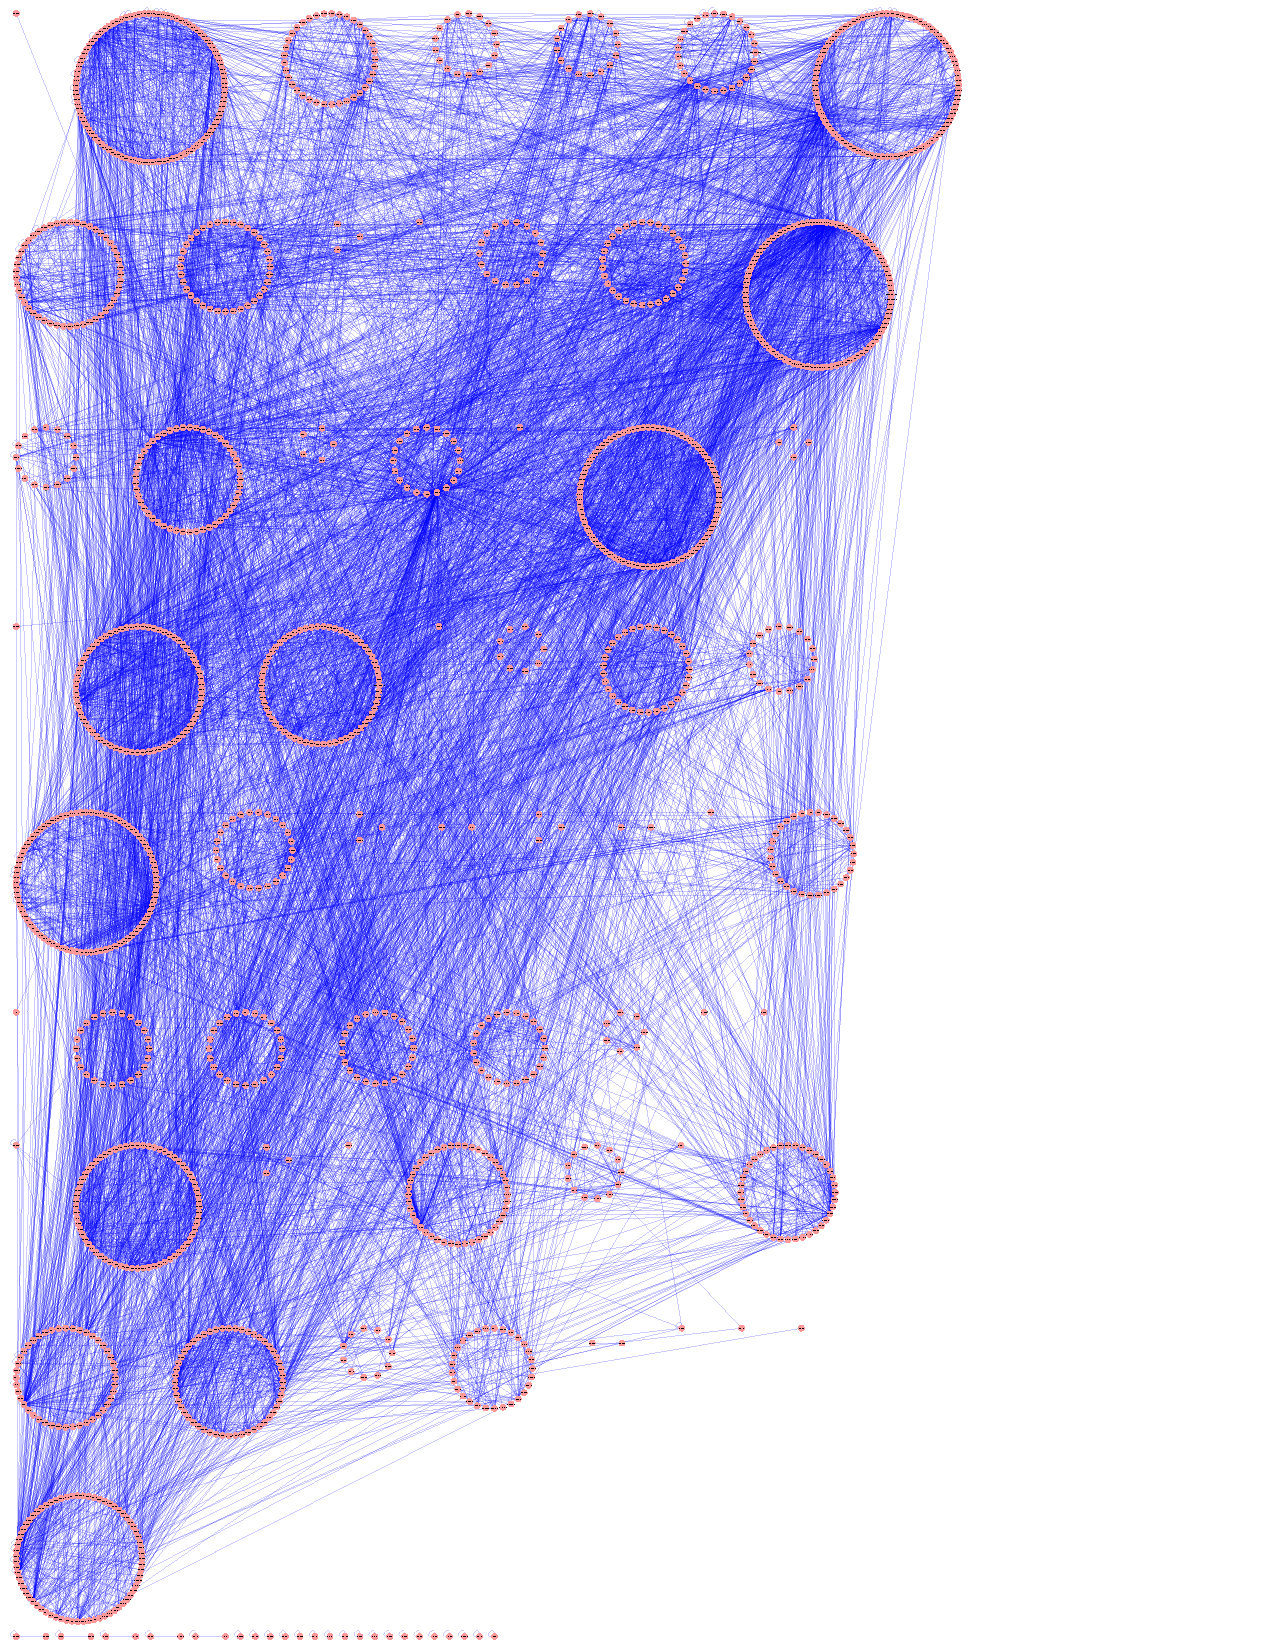
\includegraphics[width=0.8\textwidth]{unweightedgraph.pdf}
    \caption{The unweighted graph of the active zone network divided into communities.}
    \label{fig:uwgraph}
\end{figure}

\begin{figure}
    \centering
    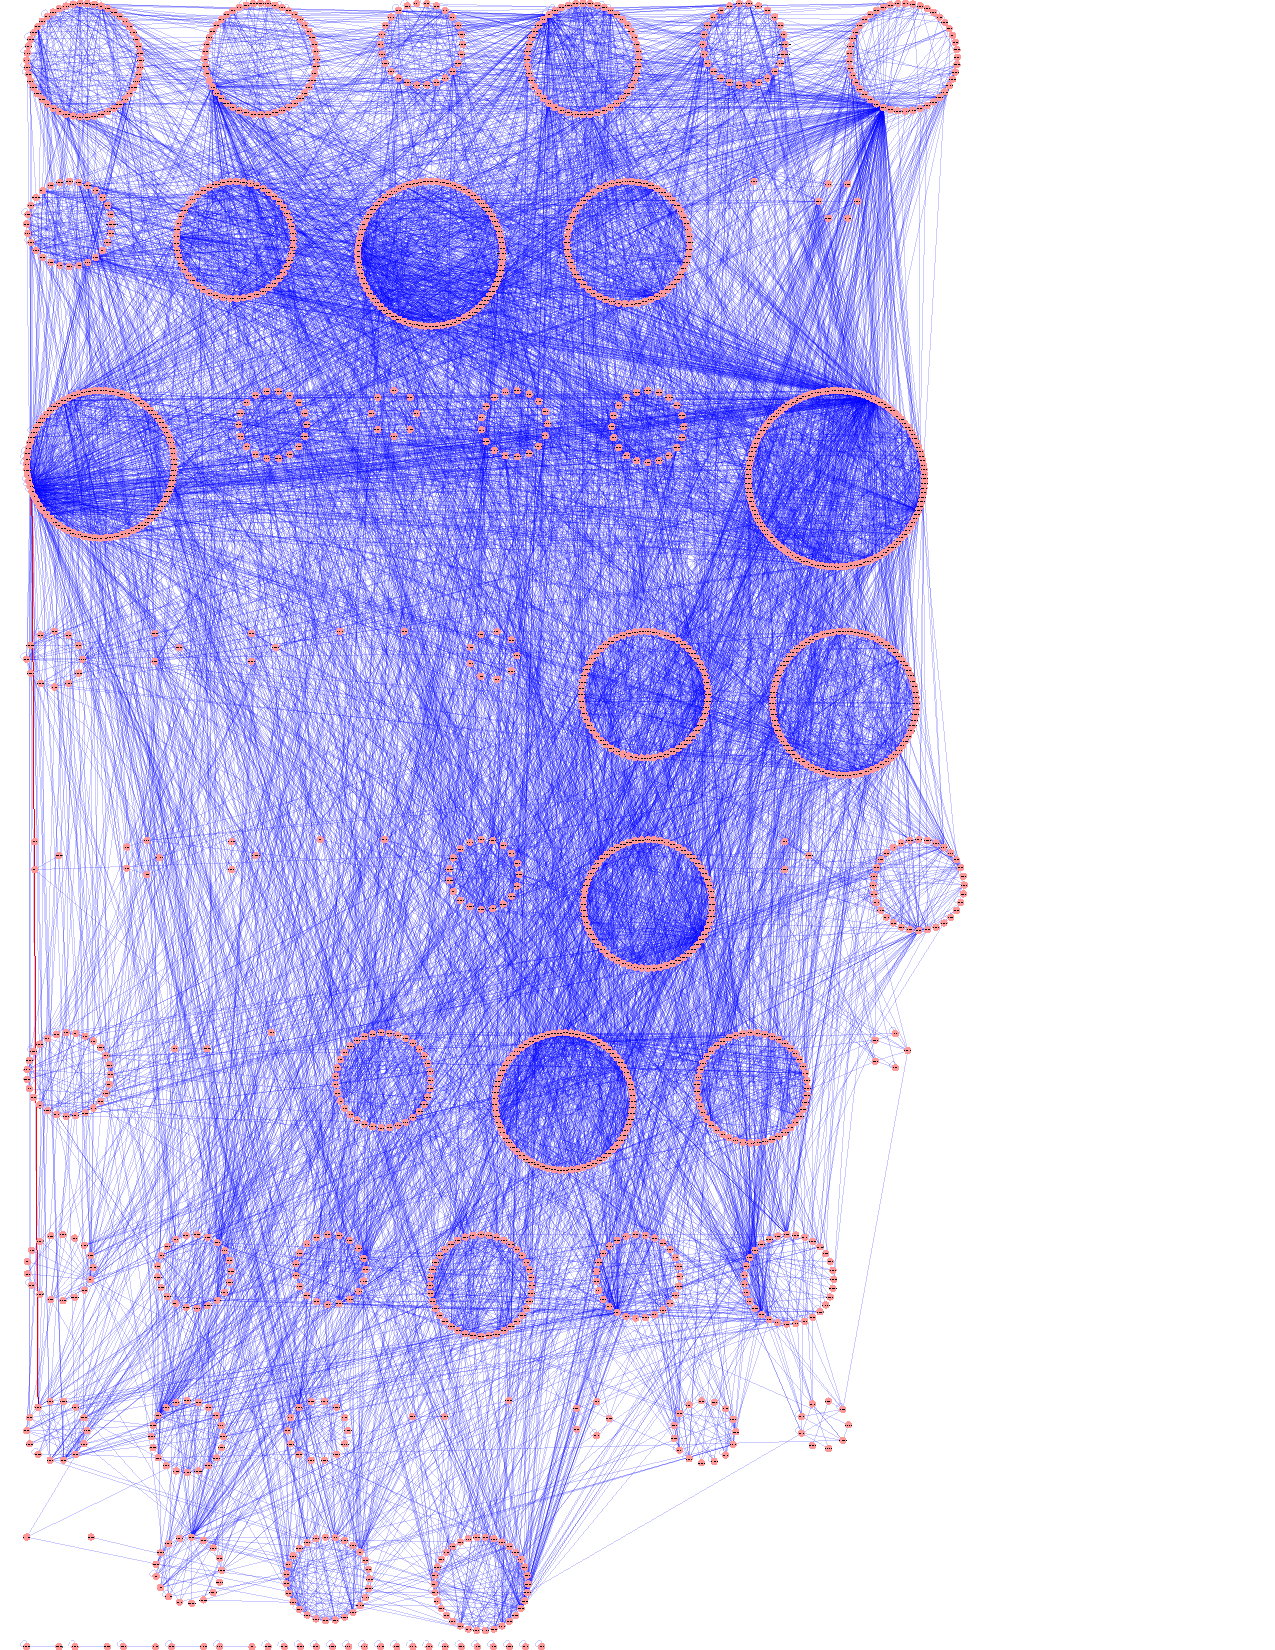
\includegraphics[width=0.8\textwidth]{weightedgraph.pdf}
    \caption{The weighted graph of the active zone network divided into communities.}
    \label{fig:wgraph}
\end{figure}

%\subsection{Graph comparison}

%comparison of using weighted and unweighted
%NMI and by eye
This observation is mirrored in the results of the NMI test.
Both NMI test implementations returned a value of 0.604, indicating that the clustering is quite similar.
%FIN: what does this mean? 
%characteristics of both graphs

\subsection{Disease enrichment}
%disease enrichment results - only schizophrenia and alzheimers to keep thing simple
The communities detected to be involved in disease differ by number between weighted and unweighted.
As these numbers are arbitrary, it is necessary to compare these communities between the two graphs to see if both graphs contain similar communities involved in disease.
%FIN: which numbers? arbitrary in what way?
The significant disease communities discovered in each graph can be found in Appendix \ref{app:disease}.

%investigate the crossover between different likely communities
Looking at the most likely community for Schizophrenia in the unweighted graph, it is possible to compare the members of this community to the members of all the communities in the weighted graph to find the closest match.
%FIN: I don't really know where the disease communities have come from SYNSYS?
Community 29 in the unweighted graph was found to be the most likely to be involved in Schizophrenia.
%FIN: according to what dataset? how? 
The membership test used equates to the number of members shared between two communities over the number of members in either community.
For this community it was found that community 33 in the weighted graph most closely matched 29 with a value of 0.45.

These graphs were then plotted to investigate the reason for this difference as shown in figure \ref{fig:nx2933}.
It can be seen that there are many more points found in the unweighted graph that are also in the weighted graph than vice versa.
In this graph it is not clear why many of these proteins have been separated, there are no clear weak connections holding together the unweighted case.
However, in figure \ref{fig:nx6444} we can see that the weighted graph contains most of the proteins of the unweighted community minus a set that are very weakly connected.

%plots
\begin{figure}
    \centering
     \setlength\figureheight{1in}
    \setlength\figurewidth{1in}
    \InputIfFileExists{\imagedir/nx2933.pgf}{}{\textbf{!! Missing graphics !!}}   
    \setlength\figureheight{1in}
    \setlength\figurewidth{1in}
    \InputIfFileExists{\imagedir/nx3329.pgf}{}{\textbf{!! Missing graphics !!}}
    \caption{The communities 29 and 33 from the unweighted and weighted graphs, respectively are plotted. In each plot the nodes not shared in each community are plotted separated from the main community on the right.}
    \label{fig:nx2933}
\end{figure}

\begin{figure}
    \centering
     \setlength\figureheight{1in}
    \setlength\figurewidth{1in}
    \InputIfFileExists{\imagedir/nx6444.pgf}{}{\textbf{!! Missing graphics !!}}   
    \setlength\figureheight{1in}
    \setlength\figurewidth{1in}
    \InputIfFileExists{\imagedir/nx4464.pgf}{}{\textbf{!! Missing graphics !!}}
    \caption{The communities 64 and 44 from the unweighted and weighted graphs, respectively are plotted. In each plot the nodes not shared in each community are plotted separated from the main community on the right.}
    \label{fig:nx6444}
\end{figure}

%relationship to functional annotations that may be linked to schizophrenia

%crossover between these communities for weighted and unweighted cases
%graphs

%characteristics of the graphs produced

%\subsection{The effect of weighting}
%weightings inside relevant communities


\section*{Conclusion}

Although it is easy to demonstrate that weighting the graph has had an effect on the communities detected, it is much more difficult to discern what this effect has been or how the weighting has brought it about.
However, many of the results presented here are positive, showing that the various techniques involved can be used to produce a result.

